\documentclass{article}
\usepackage[utf8]{inputenc}
\usepackage{enumitem}
\usepackage{cmsrb}
\usepackage{graphicx}
\usepackage[OT2,T1]{fontenc} 
\usepackage[serbian]{babel}


\begin{document}

\begin{titlepage}
    \centering

    \newcommand{\HRule}{\rule{\linewidth}{0.5mm}}
    \center
    \textup{\Large Univerzitet u Beogradu\\Matematički fakultet}\\[1.5cm]
    \textup{\Large Projekat iz predmeta Informacioni sistemi 2022/2023.}\\[0.4cm]

    \HRule \\[0.4cm]
    { \huge \bfseries Informacioni sistem srednje škole}\\[0.4cm]
    \HRule \\[1.1cm]
    
    \vspace{6 cm}
	
	\begin{minipage}{0.4\textwidth}
		\begin{flushleft} \large
			\emph{Autori:}\\
			Pavle Savić\\
			Jovan Marković\\
			Mateja Trtica\\
			Lazar Ristić\\		
		\end{flushleft}
	\end{minipage}
	~
	\begin{minipage}{0.5\textwidth}
		\begin{flushright} \large
			\emph{Predmet:}\\ 
			Informacioni sistemi\\
			\emph{Profesor:}\\ 
			Saša Malkov\\
			\emph{Asistent:}\\ 
			Dara Milojković
		\end{flushright}
	\end{minipage}\\[2cm]
	{\large \today}\\[2cm]
\end{titlepage}

\thispagestyle{empty}

\newpage
\renewcommand*\contentsname{Sadržaj:}
\tableofcontents

\newpage
\section{Slučajevi upotrebe}

\subsection{Aktivnosti Nastavnika}

\begin{figure} [!ht]
    \begin{center}
        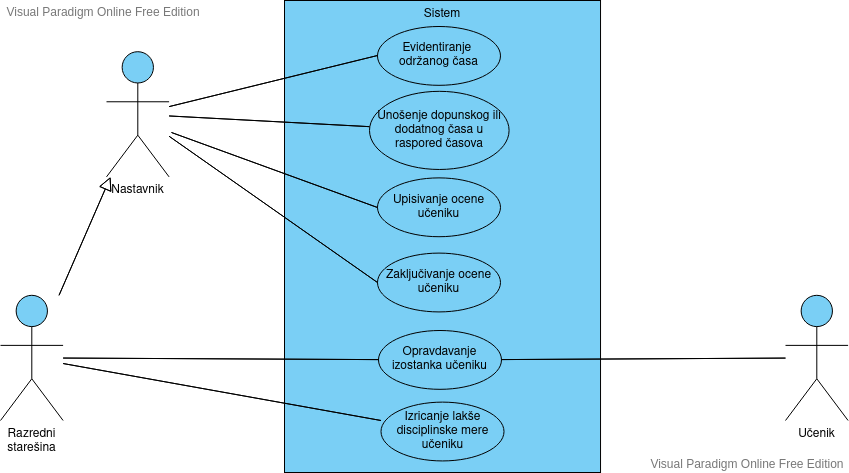
\includegraphics[scale=0.45]{imgs/nastavnik_use_case.png}
    \end{center}
\caption{Dijagram slučajeva upotrebe Nastavnika i Razrednog starešine kao njegove specijalizije}
\end{figure}

\newpage
\subsubsection{Slučaj upotrebe: Nastavnik evidentira održani čas} 
1. \textbf{Kratak opis:} Nakon održanog časa nastavnik unosi informacije o nastavnoj temi pređenoj na tom času i upisuje odsutne učenike. Sistem validira i čuva unete podatke i obaveštava nastavnika o uspešno unetom izveštaju.\\

2. \textbf{Učesnici:}
\begin{enumerate} [label=(\alph*)]
\item Nastavnik
\end{enumerate} 

3. \textbf{Preduslov:} Nastavnik je registrovani korisnik sistema. Nastavnik ima pristup Internetu. Sistem je u funkciji. \\

4. \textbf{Postuslov:} Izveštaj sa održanog časa je unet u arhivu dokumenata sistema. Odsutnim učenicima zabeležen je izostanak. Baza je ažurirana. \\

5. \textbf{Osnovni tok:} 
\begin{enumerate} [label=(\alph*)]
\item Nastavnik pristupa listi održanih časova
\item Nastavnik pritiska dugme za kreiranje novog izveštaja sa časa
\item Sistem prikazuje formular za kreiranje novog izveštaja sa časa
\item Nastavnik unosi tražene podatke 
\item Nastavnik pritiskom na dugme potvrđuje unos
\item Sistem vrši validaciju podataka
\item Sistem čuva podatke
\item Sistem vraća poruku o uspešno kreiranom izveštaju
\end{enumerate}

6. \textbf{Alternativni tokovi:}
\begin{enumerate} [label=(\roman*)]
\item Nastavnik unosi nevalidne podatke u formular - Ako u koraku (f) sistem utvrdi neispravno polje formulara sistem obaveštava nastavnika obeležavanjem nevalidnog polja. Nastavnik ispravlja neispravno polje. Proces se nastavlja iz koraka (d).
\end{enumerate}

7. \textbf{Podtokovi}: - \\

8. \textbf{Specijalni zahtevi}: - \\

9. \textbf{Dodatne informacije}: Obavezna polja formulara jesu: datum, oznaka odeljenja, nastavna tema i spisak odsutnih učenika. Opciona polja su: literatura za temu, domaći zadatak i napomene. \\


\subsubsection{Slučaj upotrebe: Nastavnik unosi dopunske i dodatne časove u raspored časova } 
1. \textbf{Kratak opis:} U dogovoru sa zainteresovanim učenicima nastavnik dodaje dodatni ili dopunski čas u postojeći raspored časova. Sistem validira i čuva unete izmene i obaveštava nastavnika o uspešno ažuriranom rasporedu. \\

2. \textbf{Učesnici:}
\begin{enumerate} [label=(\alph*)]
\item Nastavnik
\end{enumerate} 

3. \textbf{Preduslov:} Nastavnik je registrovani korisnik sistema. Nastavnik ima pristup Internetu. Sistem je u funkciji. \\

4. \textbf{Postuslov:} Dopunski ili dodatni čas dodat je u raspored časova. Baza je ažurirana. \\

5. \textbf{Osnovni tok:} 
\begin{enumerate} [label=(\alph*)]
\item Nastavnik pristupa stranici na kojoj je prikazan raspored časova
\item Nastavnik pritiska na dugme ispod odgovarajućeg dana  
\item Sistem otvara formular za upis podataka o času koji se dodaje u raspored
\item Nastavnik popunjava formular traženim podacima
\item Nastavnik pritiskom na dugme potvrđuje slanje zahteva za unos časa u raspored
\item Sistem validira unete podatke
\item Sistem vrši proveru da li je došlo do preklapanja u rasporedu časova
\item Sistem čuva podatke
\item Sistem vraća poruku o uspešno ažuriranom rasporedu
\end{enumerate}

6. \textbf{Alternativni tokovi:}
\begin{enumerate} [label=(\roman*)]
\item Nastavnik unosi nevalidne podatke u formular - Ako u koraku (f) sistem utvrdi nevalidne podatke (obavezna polja ostala nepopunjena) obaveštava nastavnika obeležavanjem neispravnog polja. Nastavnik ispravlja neispravno polje. Proces se nastavlja iz koraka (d).
\item Neuspešna izmena rasporeda - Ako u koraku (g) sistem utvrdi preklapanje u rasporedu časova obaveštava nastavnika ispisivanjem časa koji se u rasporedu već nalazi u tom terminu. Nastavnik bira drugi dan i proces se nastavlja iz koraka (b).

\end{enumerate}

7. \textbf{Podtokovi}: - \\

8. \textbf{Specijalni zahtevi}: Nastavnik dodatnu/dopunsku nastavu može zakazati samo u terminu 7. časa u prvoj smeni (predčas u drugoj smeni). \\

9. \textbf{Dodatne informacije}: Obavezna polja formulara su: naziv predmeta, odeljenje, tip časa (dopunska/dodatna). Opciono polje je napomena. \\


\subsubsection{Slučaj upotrebe: Nastavnik upisuje ocenu učeniku} 
1. \textbf{Kratak opis:} Nakon održane provere znanja (pismene ili usmene) nastavnik unosi ostvarenu ocenu učenika u elektronski dnevnik. Sistem validira i čuva unetu ocenu i obaveštava nastavnika o uspešno unetoj oceni.  \\

2. \textbf{Učesnici:}
\begin{enumerate} [label=(\alph*)]
\item Nastavnik
\end{enumerate} 

3. \textbf{Preduslov:} Nastavnik je registrovani korisnik sistema. Nastavnik ima pristup Internetu. Sistem je u funkciji. \\

4. \textbf{Postuslov:} Ocena učenika uneta je u elektronski dnevnik. Baza je ažurirana.\\

5. \textbf{Osnovni tok:} 
\begin{enumerate} [label=(\alph*)]
\item Nastavnik pristupa listi učenika podeljenih po odeljenjima kojima predaje
\item Nastavnik vrši pretragu i pritiska dugme za pristup ocenama kod odgovarajućeg učenika
\item Sistem otvara stranicu sa ocenama odgovarajućeg učenika
\item Nastavnik pritiska na dugme za unos nove ocene
\item Sistem prikazuje obrazac za unos nove ocene
\item Nastavnik popunjava obrazac
\item Nastavnik pritiskom na dugme potvrđuje unos ocene
\item Sistem validira unete podatke
\item Sistem čuva unetu ocenu
\item Sistem vraća poruku o uspešno unetoj oceni
\end{enumerate}

6. \textbf{Alternativni tokovi:}
\begin{enumerate} [label=(\roman*)]
\item Nastavnik unosi nevalidne podatke u obrazac - Ako u koraku (h) sistem utvrdi nevalidnu ocenu (ocena nije od 1 do 5) ili prazno obavezno polje obaveštava nastavnika obeležavanjem neispravnog polja. Nastavnik ispravlja neispravno polje. Proces se nastavlja iz koraka (f).
\end{enumerate}

7. \textbf{Podtokovi}: - \\

8. \textbf{Specijalni zahtevi}: - \\

9. \textbf{Dodatne informacije}: Obavezna polja obrasca su: ocena i tip ocene (kontrolni/pismeni/usmeni/aktivnost). Opciono polje je napomena. \\


\subsubsection{Slučaj upotrebe: Nastavnik zaključuje ocenu učeniku} 
1. \textbf{Kratak opis:} Na osnovu ostvarenih ocena u toku školske godine nastavnik unosi zaključnu ocenu učenika u elektronski dnevnik. Sistem validira i čuva unetu ocenu i obaveštava nastavnika o uspešnom zaključivanju ocene. \\

2. \textbf{Učesnici:}
\begin{enumerate} [label=(\alph*)]
\item Nastavnik
\end{enumerate} 

3. \textbf{Preduslov:} Nastavnik je registrovani korisnik sistema. Nastavnik ima pristup Internetu. Sistem je u funkciji. \\

4. \textbf{Postuslov:} Zaključna ocena učenika uneta je u elektronski dnevnik. Baza je ažurirana. \\

5. \textbf{Osnovni tok:} 
\begin{enumerate} [label=(\alph*)]
\item Nastavnik pristupa listi učenika podeljenih po odeljenjima kojima predaje
\item Nastavnik vrši pretragu i pritiska dugme za pristup ocenama kod odgovarajućeg učenika
\item Sistem otvara stranicu sa ocenama odgovarajućeg učenika
\item Nastavnik pritiska na dugme za otvaranje obrasca za zaključivanje ocene
\item Sistem proverava uslove za zaključivanje
\item Sistem prikazuje nastavniku obrazac za zaključivanje 
\item Nastavnik popunjava obrazac
\item Nastavnik pritiskom na dugme potvrđuje zaključivanje ocene
\item Sistem validira unetu zaključnu ocenu
\item Sistem čuva unetu zaključnu ocenu
\item Sistem vraća poruku o uspešno zaključenoj oceni
\end{enumerate}


6. \textbf{Alternativni tokovi:}
\begin{enumerate} [label=(\roman*)]
\item Nastavnik pokuša nedozvoljeno zaključivanje ocene - Ako u koraku (e) sistem utvrdi da nisu ispunjeni uslovi za zaključivanje ocene (učenik nema dovoljno ocena) obaveštava nastavnika da ocenu nije moguće zaključiti. Proces se završava.
\item Nastavnik zaključuje nevalidnu ocenu - Ako u koraku (i) sistem utvrdi nevalidnu zaključnu ocenu (ocena nije od 1 do 5, prazno polje, ocena je manja od aritmetičke sredine ocena učenika) obaveštava nastavnika obeležavanjem neispravnog polja obrasca. Nastavnik ispravlja ocenu. Proces se nastavlja iz koraka (g).
\end{enumerate}

7. \textbf{Podtokovi}: - \\

8. \textbf{Specijalni zahtevi}: Ocenu moguće zaključiti samo u poslednjoj radnoj nedelji školske godine. \\

9. \textbf{Dodatne informacije}: Minimalan broj ocena učenika da bi ocena mogla da se zaključi zavisi od fonda časova odgovarajućeg predmeta i definisan je pravilnikom škole. Obavezno polje obrasca je zaključna ocena. Opciono polje je napomena. \\


\subsection{Aktivnosti Razrednog starešine}

\subsubsection{Slučaj upotrebe: Razredni starešina opravdava učeniku evidentirani izostanak}
1. \textbf{Kratak opis:} Na osnovu opravdanja koje je učenik dostavio uživo ili elektronski skenirano kroz sistem razredni starešina evidentira izostanak kao opravdan. Sistem čuva promenu statusa odgovarajućeg izostanka i o tome obaveštava razrednog starešinu. \\

2. \textbf{Učesnici:}
\begin{enumerate} [label=(\alph*)]
\item Razredni starešina
\item Učenik
\end{enumerate} 

3. \textbf{Preduslov:} Razredni starešina je registrovani korisnik sistema. Razredni starešina ima pristup Internetu. Sistem je u funkciji. Učenik je dostavio opravdanje. \\

4. \textbf{Postuslov:} Sistem je evidentirao izostanak učenika kao opravdan. Baza je ažurirana. \\

5. \textbf{Osnovni tok:} 
\begin{enumerate} [label=(\alph*)]
\item Razredni starešina pristupa stranici sa listom učenika u svom odeljenju
\item Razredni starešina pritiska na dugme za pristup korisničkom profilu odgovarajućeg učenika
\item Sistem otvara profil učenika
\item Razredni starešina pritiska na dugme za izlistavanje izostanaka učenika
\item Sistem prikazuje listu izostanaka i status svakog izostanka (opravdan/neopravdan)
\item Razredni starešina pritiska odgovarajući neopravdani izostanak
\item Sistem prikazuje dialog box (da/ne) i pita razrednog starešinu da li želi da promeni status neopravdanog izostanka
\item Razredni starešina potvrđuje promenu
\item Sistem čuva promenu statusa izostanka
\item Sistem obaveštava razrednog starešinu o uspešnoj promeni statusa izostanka
\end{enumerate}

6. \textbf{Alternativni tokovi:}
\begin{enumerate} [label=(\roman*)]
\item Razredni starešina ne potvrđuje promenu statusa izostanka - Ako u koraku (h) razredni starešina odgovori odrično ili ugasi dialog box sistem ne evidentira promenu statusa. Proces se nastavlja iz koraka (e). 
\end{enumerate}

7. \textbf{Podtokovi}: - \\

8. \textbf{Specijalni zahtevi}: Izostanak se mora opravdati u roku od dve nedelje nakon evidentiranja. Nakon isteka roka razredni starešina više nema mogućnost opravdavanja i status izostanka ostaje - neopravdan. \\

9. \textbf{Dodatne informacije}: - \\


\subsubsection{Slučaj upotrebe: Razredni starešina izriče učeniku lakšu disciplinsku meru}

1. \textbf{Kratak opis:} Na osnovu donesene odluke razredni starešina unosi u elektronski dnevnik lakšu disciplinsku meru izrečenu učeniku. Sistem validira i čuva unete podatke i o tome obaveštava razrednog starešinu. \\

2. \textbf{Učesnici:}
\begin{enumerate} [label=(\alph*)]
\item Razredni starešina
\end{enumerate} 

3. \textbf{Preduslov:} Razredni starešina je registrovani korisnik sistema. Razredni starešina ima pristup Internetu. Sistem je u funkciji. \\

4. \textbf{Postuslov:} Dokument o izrečenoj meri je unet u arhivu dokumenata sistema. Disciplinska mera učenika evidentirana je u elektronskom dnevniku. Baza je ažurirana. \\

5. \textbf{Osnovni tok:} 
\begin{enumerate} [label=(\alph*)]
\item Razredni starešina pristupa stranici sa listom učenika u svom odeljenju
\item Razredni starešina pritiska na dugme za pristup korisničkom profilu odgovarajućeg učenika
\item Sistem otvara profil učenika
\item Razredni starešina pritiska dugme za kreiranje dokumenta o disciplinskoj meri
\item Sistem prikazuje obrazac za kreiranje dokumenta o disciplinskoj meri 
\item Razredni starešina unosi tražene podatke
\item Razredni starešina pritiskom na dugme potvrđuje unos
\item Sistem vrši validaciju podataka
\item Sistem čuva podatke
\item Sistem obaveštava razrednog starešinu o uspešno izrečenoj disciplinskoj meri
\end{enumerate}

6. \textbf{Alternativni tokovi:}
\begin{enumerate} [label=(\roman*)]
\item Razredni starešina unosi nevalidne podatke u obrazac - Ako u koraku (h) sistem utvrdi nevalidno polje obrasca (prazno obavezno polje) sistem obaveštava razrednog starešinu obeležavanjem neispravnog polja. Razredni starešina ispravlja neispravno polje. Proces se nastavlja iz koraka (f).
\end{enumerate}

7. \textbf{Podtokovi}: - \\

8. \textbf{Specijalni zahtevi}: U slučaju ukora odeljenskog veća prethodno je održana sednica na kojoj je disciplinska mere izglasana. \\

9. \textbf{Dodatne informacije}: Obavezna polja obrasca jesu: datum, nivo mere (opomena/ukor razrednog starešine/ukor odeljenskog veća), razlog izricanja mere. Opciono polje je napomena. Lakše disciplinske mere ne povlače smanjenje ocene iz vladanja. Odeljensko veće čine nastavnici koji izvode nastavu u određenom odeljenju. \\


\end{document}